\documentclass[journal]{IEEEtran}
\usepackage{graphicx}
\usepackage{booktabs}
\usepackage{tabularx}
\usepackage{array}
\usepackage{url}
\usepackage[hidelinks]{hyperref}
\title{Supplementary File S5: Experimental Protocol and Evidence Ledger}
\author{}
\begin{document}
\maketitle

\noindent This supplement documents the latest available system-integration
evidence and its limits. The runs below were performed against local virtual
industrial endpoints. Evidence units are kept separate because they differ in
task, actor, runtime configuration, and endpoint state. The associated
machine-readable records and original CSV exports are supplied in
\texttt{Supplementary-File-S5-Evidence.zip}. A companion HTML audit report
provides an interactive step-by-step view.

\section{Evidence Scope and Separation}
The primary case is the completed 2026-10-31 document-driven HTTP/MQTT
integration. It evaluates interface mapping, acquisition, read-only lead-task
execution, and export consistency. The setpoint write/readback check was
operator initiated and is reported separately from the agent task. Other
model-backed, AgentTeam, protocol, and process-mission records are independent
supporting evidence; counts and trajectories are not pooled. No physical plant
was connected.

\section{Document-Driven Virtual Integration}
\subsection{Configuration and execution}
An interface contract declared six signals: HTTP enclosure temperature PV,
setpoint, setpoint readback, and a 64-point thickness profile; and MQTT
ambient temperature and humidity. The configuration created one new line,
five DAQ nodes, one DCW node, a product, and a recipe. Provisioning reported
11/11 checks passed and zero cross-line write-point conflicts. The resulting
Channel contained a lead and three configured worker roles. The archived
activation evidence verifies only the lead as wired, and the retained task
was assigned to that lead. The task was read-only and terminated
\texttt{COMPLETED} at 100\%.

\subsection{Acquisition and export}
The lead task queried five acquisition streams: four scalar signals and the
vector profile. The task record contains 17 aggregated buckets for each scalar
signal and 22 profile frames, each with 64 points. The observed ranges and
export checks are summarized in Table~\ref{tab:s5-read}. Scalar query buckets
and exported CSV rows have different aggregation semantics and must not be
added together. The 19/19 export checks verify headers, manifest counts, value
ranges, and vector shape. The CSV archive includes startup rows marked
\texttt{offline}; thus, contract consistency does not imply that every row is
a valid online observation.

\begin{table}[!t]
\centering
\caption{Read-only task observations and exported data.}
\label{tab:s5-read}
\footnotesize
\setlength{\tabcolsep}{3pt}
\begin{tabularx}{\columnwidth}{@{}>{\raggedright\arraybackslash}p{1.28cm}>{\raggedright\arraybackslash}p{1.12cm}X@{}}
\toprule
Signal & Task coverage & Observed range or structure \\
\midrule
Enclosure PV & 17 buckets & 24.515--25.480\,$^{\circ}$C; mean 25.052\,$^{\circ}$C \\
SP readback & 17 buckets & 25.0\,$^{\circ}$C throughout the task window \\
Thickness profile & 22 frames & 64 points/frame; frame means 2.4975--2.5041\,mm \\
Ambient temperature & 17 buckets & 20.5--23.44\,$^{\circ}$C \\
Ambient humidity & 17 buckets & 50.0--59.8\% \\
\midrule
Scalar CSVs & 818 rows & Four files; includes startup offline rows \\
Vector CSV & 3,456 rows & 54 frames $\times$ 64 points/frame \\
Export validation & 19/19 & Manifest, headers, counts, ranges, and shape checks \\
\bottomrule
\end{tabularx}
\end{table}

\subsection{Independent write/readback check}
The virtual line began at a recipe setpoint of 25\,$^{\circ}$C. An early
operator request for 27\,$^{\circ}$C was rejected because the 60-s write
interval had not elapsed. A later operator/controller check wrote 27 and
restored 25. A separate DAQ node observed both values. The HTTP write response
echoed the request and is not treated as device readback. The write records
have no task, approval, actor, or driver-event identifier linking them to the
read-only agent task. This sequence therefore demonstrates an independent
simulator write/readback path, not agent-controlled actuation.

\begin{figure*}[!t]
\centering
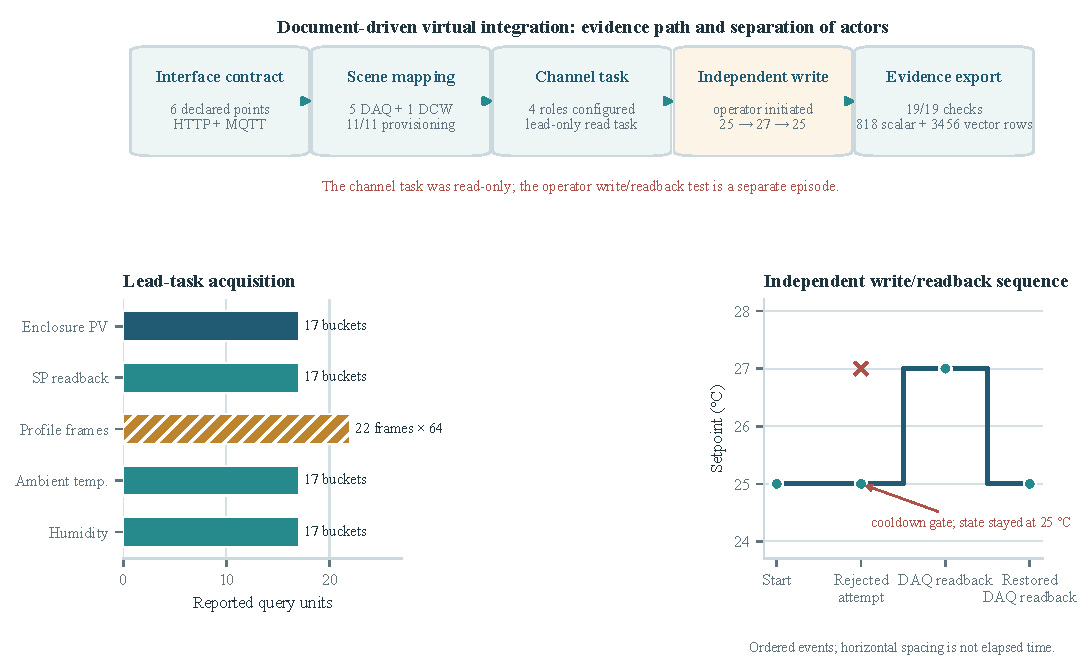
\includegraphics[width=0.94\textwidth]{resources/fig-latest-doc-driven-integration.pdf}
\caption{Evidence sequence for the document-driven virtual-line case. The
read-only lead task and operator-initiated writes are intentionally shown as
separate paths. The lower panels summarize the retained scalar buckets,
vector frames, and ordered setpoint observations. Horizontal spacing denotes
event order only, not elapsed time or a causal trajectory.}
\label{fig:s5-integration}
\end{figure*}

\section{Latest System Regression Results}
Table~\ref{tab:s5-tests} summarizes the 2026-10-31 T0--T4 acceptance report.
These software and integration checks are not repeated process trials.

\begin{table*}[!t]
\centering
\caption{Latest system regression checks and scope.}
\label{tab:s5-tests}
\footnotesize
\setlength{\tabcolsep}{4pt}
\begin{tabularx}{\textwidth}{@{}p{1.5cm}X p{2.2cm}@{}}
\toprule
Stage & Result & Qualification \\
\midrule
T0 static & Lint passed after five existing lint errors were fixed; typecheck, documentation, localization, and README checks passed. & Completed after repair and rerun \\
T1 unit/contract & Unit: 915 tests, 913 passed, 0 failed, 2 skipped; MCP 14/14; plugin lifecycle 22/22; SDK surface passed; twin provider 5/5; skills 147/147. & Software checks only \\
T2 core integration & Line governance 44/44; document-driven virtual integration passed within the scope in Section II. High-load ontology, optimizer, UI, and model suites were not run in this campaign. & Limited coverage \\
T3 API-live & No qualified run: the script's fresh-instance registration precondition was unmet on the already-used service; other T3 suites were not run. & Not counted as pass or product failure \\
T4 plugin/tool surface & 11 plugins with zero reported failures; 126/126 registered tools available. & Registry availability, not per-tool E2E \\
\bottomrule
\end{tabularx}
\end{table*}

\section{Separate Agent, Route, and Protocol Evidence}
Table~\ref{tab:s5-runs} lists independent runs that are not combined with the
primary integration case.

\begin{table*}[!t]
\centering
\caption{Separate evidence records and their admissible interpretation.}
\label{tab:s5-runs}
\footnotesize
\setlength{\tabcolsep}{4pt}
\begin{tabularx}{\textwidth}{@{}p{2.2cm}X p{3.3cm}@{}}
\toprule
Run & Recorded result & Interpretation \\
\midrule
OMP/Qwen, 2026-10-30 & R3: setpoint stayed at 195 while a scripted approval was pending, then read 198 after approval. R4 wrote 200.5; the retained PV observation was 199.45. The simulator was already running. & One script-approved simulator write path and one later bounded write; not human-review efficacy or process improvement. \\
Qwen R2 query assertion & Original runner marked R2.1 pass; the task was \texttt{CANCELED}, and its deliverable values did not match the queried value. The assertion searched arbitrary numbers in full task history. & Query success is unverified and excluded. The earlier consolidated values 207.67/205.83 and 200.84 are not supported by the retained JSON. \\
OMP / USTC--DeepSeek-configured, 2026-10-31 & Four tools were invoked and 50 DAQ points were recorded; acceptance was 10/13 and the task remained \texttt{WORKING}. No approval or successful write was retained. Runtime model attestation is absent. & Incomplete exploratory task; not an A2 model result. \\
P12 AgentTeam, 2026-10-30 & Qualification passed; workflow and evidence-integrity gates failed. The task was canceled on a stale/future sample; no verified approvals or accepted writes; worker dispatch not verified. & Not a successful team episode. \\
Route fixture & Four deterministic simulator transitions with matching separate reads: cast-film 120 to 125/130 rpm and annealing 730 to 735/740\,$^{\circ}$C; synthetic administrator approval; no agent-selected action or post-write process response. & State-transition checks only. \\
Protocol matrix, 2026-10-29 & Five local simulator protocols; 52 acquisition samples; four write-capable protocols; 24/24 out-of-window probes rejected; LLM disabled. & Deterministic protocol/guard checks only. \\
A1/A2 & Approval-only ablation and full Harness$\times$model matrix remain \texttt{NOT-RUN}; runner is not implemented. & No causal approval, harness, or model comparison is available. \\
\bottomrule
\end{tabularx}
\end{table*}

\section{Four Scripted Process Missions}
The September 28 mission records provide additional multi-scene simulator
coverage. Each row is one deterministic trajectory; scripted routines, rather
than an LLM, selected setpoints. These trajectories are not replications of
the October document-driven integration and do not isolate causal action
effects. Some terminal secondary variables were not archived.

\begin{table}[!t]
\centering
\caption{Reported primary values in the four scripted missions.}
\label{tab:s5-missions}
\footnotesize
\setlength{\tabcolsep}{3pt}
\begin{tabularx}{\columnwidth}{@{}>{\raggedright\arraybackslash}p{1.28cm}X@{}}
\toprule
Scene & Target band; initial $\rightarrow$ reported final \\
\midrule
Injection & 32.15--32.85\,g; 31.296 $\rightarrow$ 32.36\,g \\
BOPET film & 24.3--25.7\,$\mu$m; 28.03 $\rightarrow$ 25.30\,$\mu$m \\
Annealing & 89--101\,HV; 134.9 $\rightarrow$ 99.5\,HV \\
Wastewater & 2.8--4.0\,mg/L DO; 0.194 $\rightarrow$ 3.54\,mg/L \\
\bottomrule
\end{tabularx}
\end{table}

\section{Evidence Completeness and Manuscript Use}
The primary integration case supports a bounded claim that a declared
HTTP/MQTT virtual scene can be mapped into configured acquisition/control
nodes, queried by a completed lead task, and exported with checked
manifest/vector structure. The separate DAQ observations support one
operator-initiated simulator write/readback demonstration. Software test
counts support tested implementation paths. These data do not demonstrate
multi-agent collaboration, approval-only causal effects, harness/model
equivalence, repeated-run process performance, or physical deployment.

All source evidence used for the summary is copied without transformation
where marked so in \texttt{SOURCE-MANIFEST.json}; original and delivered
SHA-256 hashes are listed there and in \texttt{SHA256SUMS}. The original
document-driven archive did not contain a contemporaneous checksum manifest;
the package hashes establish integrity of the delivered copy, not a
run-time-signed provenance chain. The audit report provides the step-by-step
timeline, CSV row audit, and source-file hashes. The detailed machine
records, run logs, exports, and correction to the earlier Qwen acceptance
summary are included in the evidence ZIP.

\end{document}
